\section{Introduction}

\begin{figure*}[!t]
    \centering
    %\vspace{-10pt}
    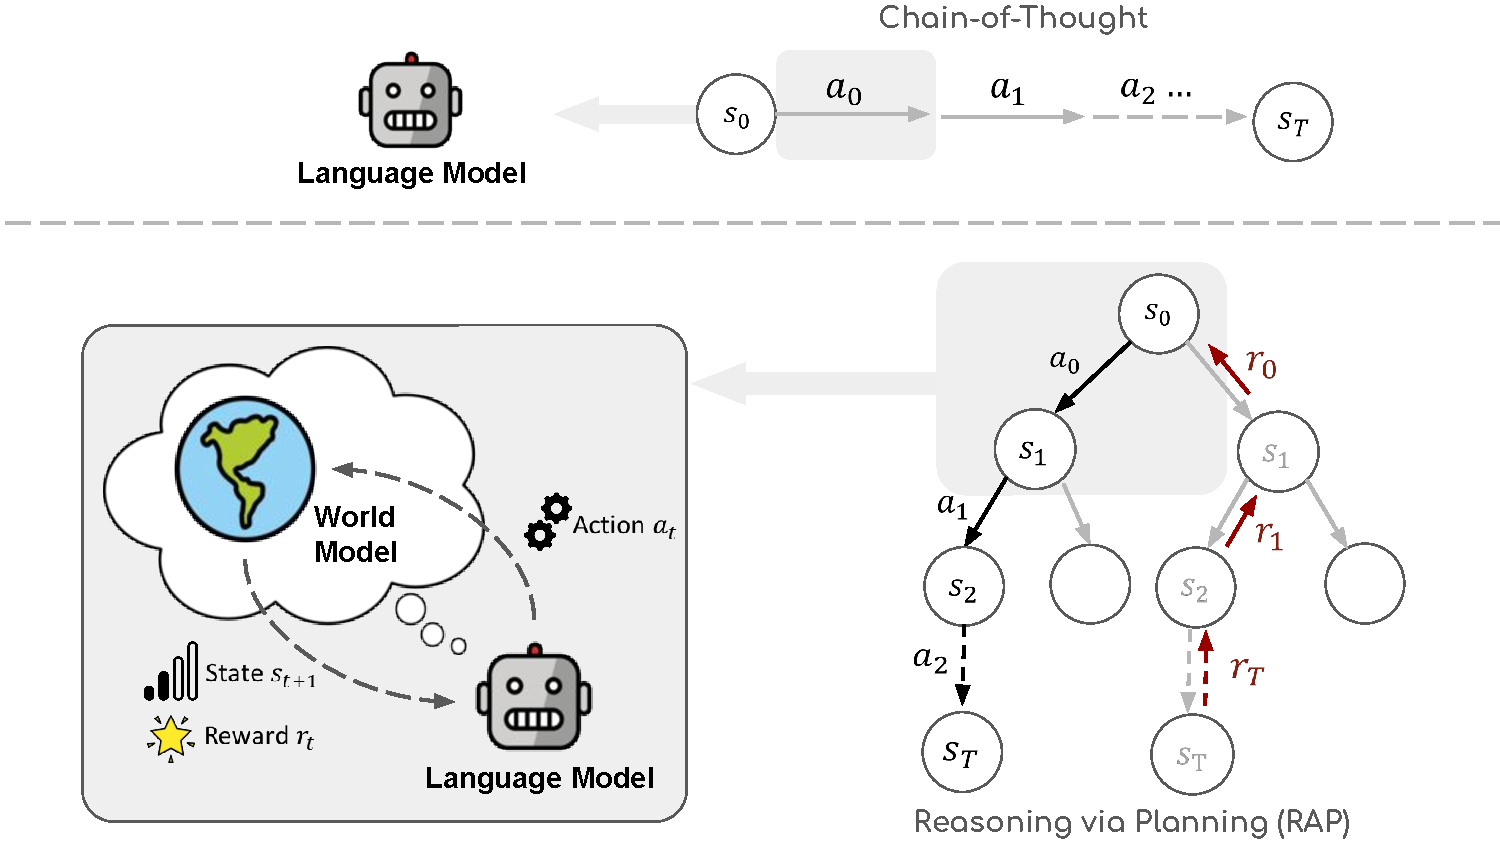
\includegraphics[width=0.8\textwidth]{sections/Figure-1_final.pdf}
    %FIGURE 1
    \vspace{-8pt}
    \caption{An overview of Reasoning via Planning (RAP). Compared with previous LLM reasoning methods like Chain-of-Thought \cite{wei2022chain}, we explicitly model the world state from a world model (repurposed from the language model), and leverage advanced planning algorithms to solve the reasoning problems.
    }
    \label{fig:1}
    \vspace{-12pt}
\end{figure*}


Large language models (LLMs) have exhibited emergent reasoning abilities in a wide range of tasks~\cite{brown2020language, chowdhery2022palm, openai2023gpt4}. Recent approaches further boost their ability by prompting LLMs to generate intermediate reasoning steps, e.g., Chain-of-Thought, CoT \cite{wei2022chain} or answer a series of subquestions, e.g., least-to-most prompting \cite{zhou2022least}. However, LLMs still face difficulties with tasks that humans find easy. For example, in creating action plans to move blocks to a target state, GPT-3 \cite{brown2020language} achieves a success rate of only 1\%, compared to 78\% for humans \cite{valmeekam2022large}; these models also struggle with complex tasks that require multiple steps of math, logical, or commonsense reasoning~\cite{ huang2022towards, mialon2023augmented}.

Humans possess an internal {\bf world model}, a mental representation of the environment~\cite{johnson1983mental, johnson2010mental, gentner2014mental}, which enables humans to simulate actions and their effects on the world's state for deliberate {\bf planning} for complex tasks of motor control, imagery, inference, and decision making \cite{tolman1948cognitive, briscoe2011mental, schulkin2012action, lecun2022path}. For example, to make an action plan towards a goal, planning with the world model involves exploring various alternative courses of actions, assessing the likely outcomes by rolling out possible future scenarios, and iteratively refining the plan based on the assessment~\cite{huys2012bonsai, gasparski2014designology, ho2021control}. This is in stark contrast to the current LLM reasoning, which instinctively generates a reasoning trace in an autoregressive manner. In particular, we identify several key limitations of the current reasoning with LLMs, including {\bf (1)} the lack of an internal world model to simulate the \emph{state} of the world (e.g., the configuration of blocks, the values of intermediate variables),
%~\cite{kratzer2007situations, zwaan2012revisiting, li2022language}), 
which is the foundation of human planning; {\bf (2)} the absence of a \emph{reward} mechanism to assess and guide the reasoning towards the desired state; and due to both limitations, {\bf (3)} the incapability of balancing \emph{exploration vs. exploitation} to efficiently explore vast reasoning space.


To address these limitations, this paper proposes a new framework, {\bf Reasoning via Planning (RAP)}, that enables LLMs to reason in a manner close to humans' conscious planning. \ours augments the LLM with a world model, and reasons with principled planning (specifically \emph{Monte Carlo Tree Search, MCTS}) to produce high-reward reasoning traces after efficient exploration (Figure~\ref{fig:1}). Notably, we acquire the world model by repurposing the LLM itself with appropriate prompts. During the reasoning, the LLM strategically builds a reasoning tree by iteratively considering the most promising reasoning steps (\emph{actions}) and using the world model (the same, repurposed LLM) to look ahead for future outcomes. The estimated future rewards are then backpropagated to update the LLM's beliefs about the current reasoning steps, guiding it to refine the reasoning by exploring better alternatives. Our MCTS-based planning effectively maintains a proper balance between exploration (of unvisited reasoning traces) and exploitation (of the best reasoning steps identified so far). 
%\hzt{Mention Aggregation here or in the experiment paragraph?}
%Aggregation is only used once and the result is not very impressive. Maybe skip it in intro
%\hsb{Compared with two concurrent works on advanced searching algorithms over the reasoning space (Guided beam search \cite{xie2023decomposition} and Tree-of-thoughts \cite{Yao2023TreeOT}), our framework stands out as a more comprehensive solution, encompassing them as a superset while also offering distinct advantages, such as the explicit state modeling, look ahead and efficient exploration.}\hzt{This is too vague. Let's discuss}

\begin{figure*}[!t]
    \centering
    %\vspace{-5pt}
    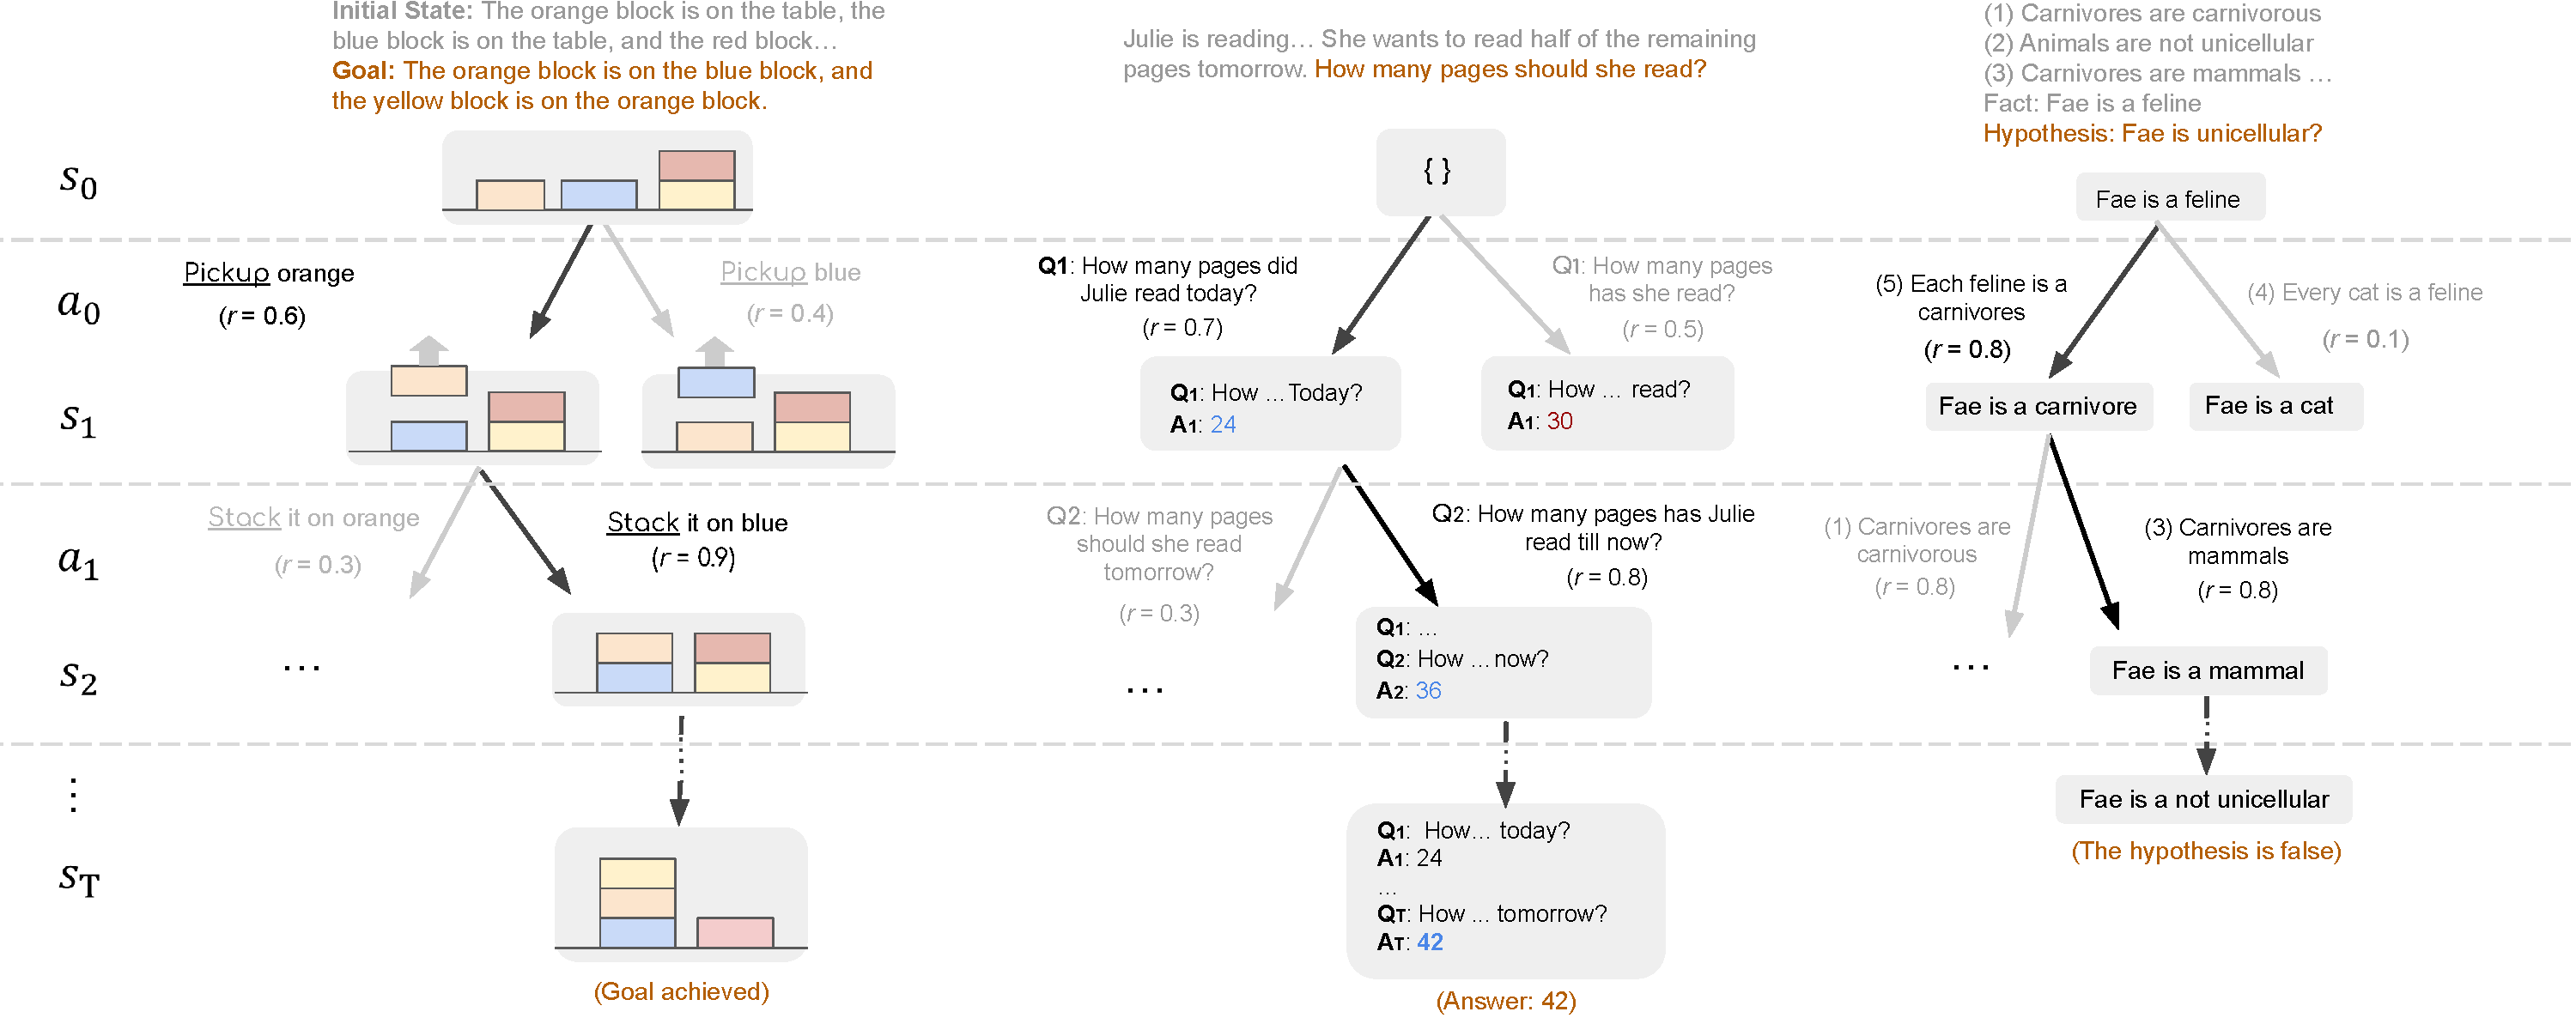
\includegraphics[width=\textwidth]{sections/Figure-2_final.pdf}
    \vspace{-22pt}
    \caption{RAP for plan generation in \blocksworld (left), math reasoning in GSM8K (middle), and logical reasoning in PrOntoQA (right).}
    \label{fig:tree_examples}
    \vspace{-15pt}
\end{figure*}

% Extensive experiments on a diverse range of challenging reasoning problems demonstrate the effectiveness of \ours by substantial improvements over various strong CoT-based reasoning approaches and even GPT-4. 
% We show that as a general reasoning framework, \ours enables a flexible formulation of rewards, states, and actions for solving distinct tasks. 
We show RAP is a general framework applicable to a diverse range of challenging problems and achieves substantial improvements over recent popular LLM reasoning methods.
For plan generation, particularly in 2/4/6-step problems of \blocksworld \cite{valmeekam2023planning}, RAP achieves an average success rate of 64\% while CoT fails almost completely. Moreover, LLaMA-33B with RAP surpasses GPT-4 with CoT by 33\% relative improvement.
In the domains of mathematical reasoning, such as GSM8K \cite{cobbe2021training} and logical inference exemplified by PrOntoQA \cite{saparov2022language}, \ours also consistently improves over strong baselines, including CoT, least-to-most prompting, and their self-consistency variants.
% beats the best CoT-based baselines by $6.8\%$ and $4.4\%$ accuracy improvement on GSM8K \cite{cobbe2021training} and PrOntoQA \cite{saparov2022language}, respectively.
 


% a diverse range of challenging problems in distinct settings, including action plan generation in a given environment , math word problems , and multi-step logical reasoning with provided logical rules (e.g., PrOntoQA \cite{saparov2022language}). RAP offers effective solutions to problems by instantiating states, actions (reasoning steps), and rewards. 
% Experiment results demonstrate substantial improvements in RAP over a range of popular reasoning approaches. On \blocksworld, \hzt{Please summarize key results}.


%\hzt{Mention previous methods as special cases?}
% maybe better mention them in the last paragraph?

% assess, roll out, 

% state, exploration/exploitation, reward/value

% plan generation (desired target state), QA (final answer)





%% ============== V1 =================


%Large language models (LLMs) \cite{brown2020language,chowdhery2022palm, touvron2023llama, openai2023gpt4} have exhibited remarkable ability across various domains, spanning abstraction, comprehension, vision, coding, mathematics, medicine, law, and understanding of human emotions \cite{bubeck2023sparks}. These exciting breakthroughs prompt researchers to consider whether these LLMs can be seen as Artificial general intelligence (AGI) \cite{bubeck2023sparks} \hzt{This paragraph is irrelevant to our work. There is no point to mention "AGI"..}. 
%However, when we compare LLMs with the human brain, it becomes apparent that current autoregressive Transformers \cite{vaswani2017attention} have an over-simplified architecture. \citet{lecun2022path} propose a conceptual architecture for AGI inspired by cognitive science and neuroscience, consisting of a configurator module, a short-term memory module, a perception module, a world model module, an actor module, and a cost module \hzt{I don't think we need to motivate ours by LeCun's paper/claims. We don't even need to mention LeCun. Perhaps fine to mention it briefly in Related Work.}. While Transformers may fit these modules implicitly during pre-training, \hzt{All the text before this point is irrelvant. We can even start the section with the following sentence.} there is evidence to suggest that current LLMs struggle with complex tasks that require the clear specification of different modules. For instance, \textbf{planning} tasks \cite{valmeekam2022large} highlight this issue \hzt{What do we mean by "planning" specifically? Need concrete examaples to articulate. Also, our work is to solve "reasoning" with the "planning" method. So "planning" is a method, not a problem to solve. Use "reasoning" to describe those problems.}.
%Until the planning is completed, an agent \gy{emphasize ``autoregressive LLM''} \hsb{Here I just want to introduce the setting of a general planning problem} is not able to interact with the real world, so it can only "guess" the results of a potential action. Additionally, a criterion is in need to evaluate and select potential actions. These two functionalities, namely the ability to predict \textbf{state transition} and to evaluate actions by providing \textbf{reward}, are primarily handled by the world model. The well-known shortage of current LLMs in planning \cite{valmeekam2022large, bubeck2023sparks} could be explained by their lack of a \textbf{world model} \cite{henaff2017model, lecun2022path, ha2018world}. \hzt{Need to introduce/motivate the concept of "world model" in a better way.}
%Given their demonstrated ability to encode rich commonsense knowledge \cite{west2021symbolic}, this failure may not be due to the ignorance of LLMs about the world,  Rather, the more plausible explanation is that the end-to-end training of LLMs doesn't encourage specialization of the world model \hzt{What does "specialization of the world model" mean?}. As such, it is worth exploring whether explicitly instructing LLMs to perform two separate roles - one as the agent and the other as the world model - results in better planning \hzt{Motivation too weak/unclear.}.



%%% ============= V2 ==============



% Large language models (LLMs) \cite{brown2020language,chowdhery2022palm, touvron2023llama, openai2023gpt4} have exhibited remarkable reasoning ability across various domains, but their ability for long-range reasoning is still very limited \cite{valmeekam2023planning} compared to humans. For example, in Blocksworld, where an agent is expected to generate an action sequence to move some blocks to a desired state, GPT-3 \cite{brown2020language} only reaches 1\% of accuracy, while humans can manage to get 78\% success rate. Given the fact that the latest LLMs reach human-level performance in many tasks, even passing a bar exam \cite{openai2023gpt4}, the failure on this commonsense task is conspicuous and prompts a question: Is long-range reasoning the Achilles' Heel of LLMs? \hsb{Keep track of state. Explain the state. Concrete examples. Reward. Guide.}

% \hsb{use the limitation as motivation. don't use other domains}
% We may get some inspiration from how people reason: Researchers in psychology and cognitive science found people use \textbf{world models} \cite{craik1967nature} that can predict the plausible state of the world. When faced with long-range reasoning task, instead of straightforwardly proposing a reasoning trace, humans may do \textbf{planning} in their mind by imagining different actions and their potential outcomes \cite{lecun2022path, kahneman2011thinking}. This procedure is also applied in optimal control \cite{bryson1975applied} and recent reinforcement learning research \cite{ha2018world}. However, most LLMs are based on autoregressive transformers and lack selective bias towards this mindset \hsb{system-2?}, which may account for their failure on reasoning tasks.

% \hsb{previous method: cot/least to most}

% In this work, we propose a novel framework to solve the reasoning via planning. We attempt to utilize the LLM as both an agent and a world model. At each reasoning step, the agent proposes some possible actions, while the world model predicts the next state and a reward. The feedback from the world model guides the agent LLM to strategically plan in two senses: (1) Given a predicted world state, it's easier for the agent LLM to propose the following actions because the remaining problem requires shorter reasoning paths (2) With the reward, we can apply Monte-Carlo Tree Search to efficiently explore and exploiting possible reasoning paths. 
% \hsb{special cases}

% \hsb{figure 1}


%While LLMs can be used as world models in classic planning problems straightforwardly, their flexibility to respond to any natural language queries enables them to address more \textbf{open} problems. Moving beyond classic planning, we explore \textbf{multi-step reasoning} by framing them as planning problems. Here, a world state is defined as a set of known variables. The agent proposes an unknown variable to reveal at each step, and then the world model reasons over its value and expands the known variable set \hzt{Unclear what do "variables" mean? What do "unknown/known" mean?}. A reward is also estimated based on its confidence and the usefulness of the reasoning step. In this context, the world model serves as an interface that encapsulates the LLM's more general understandings of the world, e.g. arithmetics and relational reasoning, rather than being limited to physical common sense.

%By formulating these planning problems within the reinforcement learning setting, we can leverage planning algorithms to solve them, such as Monte-Carlo Tree Search (MCTS). When a partial plan appears to be "promising", the agent is encouraged to revisit and continue it, while hopeless plans are discarded in favor of exploring new planning paths. 

%In the classic planning problem blockworld, our method achieves state-of-the-art performance with a substantial leap over the baseline. In multi-step reasoning problems including GSM-8k \cite{cobbe2021training} and StrategyQA \cite{geva2021did}, our method is comparable to previous sample-then-aggregate approaches like self-consistency \cite{wang2022self} with only one single path. Additionally, the human evaluation shows that our method produces more favorable paths than the baselines. \hsb{This paragraph is temporary and subject to our final results}

%In summary, we suggest using LLMs as explicit world models for planning, formulating classic planning and multi-step reasoning problems \cite{cobbe2021training, geva2021did} in an RL setting, and applying MCTS. We achieved state-of-the-art results in classic planning problems, and our proposed method outperforms previous approaches in multi-step reasoning problems. Our approach validates the need for a specialized world model to assist agents in planning, which we hope can inspire future research toward a more human-like architecture of AGI.


%We begin by focusing on \textbf{classic planning} problems, specifically represented by the blockworld \cite{valmeekam2022large}, where the agent is expected to generate an action plan to operate some blocks from an initial state to the goal state.\hsb{refer to figure 1 here} The world model serves to predict the state of the physical world so that the agent can base its future actions on the current world state. Moreover, the world model provides feedback on potential actions, such as whether they are legal or whether the new state is closer to the goal. 
%We first apply our framework to a classic plan generation task, Blockworld \cite{valmeekam2023planning}. Given a set of piles of blocks, a robot can take a sequence of actions (e.g. \textsc{stack}, \textsc{pickup}, etc.) to arrange blocks into a specified target configuration. We prompt the world model LLM to perform two jobs: (1) evaluate the action about its validity (2) describe the state of blocks given a possible action, and (3) decide whether the new state is closer to the goal state. The predicted state is appended to the prompt for agent LLM so that it can be more informed when proposing the next actions, while the rewards serve as the signals for choosing the node to expand in MCTS. 
